\documentclass[12pt]{article}
\usepackage[english]{babel}
\usepackage{amsmath,amsthm}
\usepackage{graphicx}
\usepackage{amsfonts}
\usepackage{indentfirst}
\usepackage{lscape}
\usepackage[top=2.5cm,bottom=2.5cm,right=2.5cm,left=2.5cm]{geometry}
\usepackage{titlesec}
\setcounter{secnumdepth}{5}

% ----------------------------------------------------------------
\begin{document}

\section{Process flow}

What we call process flow in this project is the main function of the project. Indeed in that function we have to manage almost all the others function, and more precisely features function, classification function, test and validation function, or create or manage the directory files.
This program is make that we can change the different descriptors (SIFT C$_2$O) as we want.
In this part we will present how works the sub-functions inside the process flow.

\subsection{Workspace}

The aim of the Process flow function is to allow at the user to choose his workspace, and choose where he want to write the results obtained by the software. Here we can see how the folder will be organize by using this function:

\begin{figure}[h]
    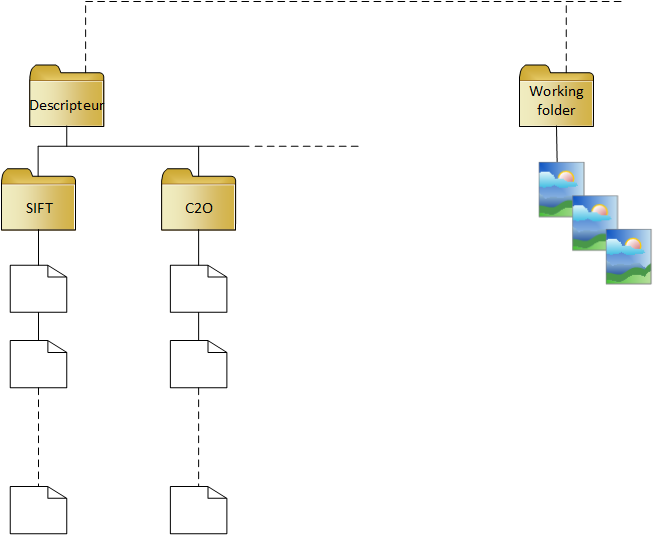
\includegraphics[scale=0.7]{arborescence.png}
    \caption{Organization of the workspace}\label{fig:process1}
\end{figure}

 Indeed we can see that we create a folder descriptor, if he is not create yet, in this folder we create as much folders as the user wants. For this he just has to enter the name he wants in the parameter \textit{name\_desc}. We can also see, the user can choose the work folder he wants.

\subsection{processing}

The second goal of this function is to compile the whole processing, so if the user wants to compile one particular function in the software he should not use the function \textit{Process\_flow}. In this function we will found this line-up:

\begin{itemize}
\item Creation of folders and path to the workspace 
\item Calculation of descriptors and link with IDs for the training database.
\item Writing descriptors in text files.
\item Calculation of K-means.
\item Signature design for whole images.
\item Classification of the test database using the K-nn method. 
\end{itemize}

The schedule project does not allow us to optimize all the function, so we can see that the K-means function take long time. To solve this problem, and if you want to test the same signature (same descriptor, and same number of words), we have made an option for use the last dictionary you calculate before.

% ----------------------------------------------------------------
\end{document} 